\section{Introduction}

\begin{frame}
	\frametitle{Discretization}
	\begin{block}{Use of discretization}
		Many systems in the real world are continous systems: chemical reactions, rocket trajectories, power plants, ice cap melting... Computers, however, are mainly digital. If we want to simulate the continuous system with a digital device, we need a method to convert the continuous model into a discrete one.  This conversion is called "discretization" or "sampling". Discretization also comes in handy when a continuous filter with usefull properties has been designed and a discrete filter with the same properties is required.
	\end{block}
\end{frame}

\begin{frame}
	\frametitle{Discretization}
	\begin{block}{Problem statement}
		While converting, some information of the continuous model may be lost due to the different nature of the systems. It is important that the loss of information is minimized. Each discretization method has its own qualities and they will all lead to different discrete representations of the same continuous system.
	\end{block}
	
	\begin{block}{Discretization methods discussed in this lecture}
		\begin{itemize}
			\item Numerical Integration
			\item Zero-pole equivalent
			\item Hold equivalents
		\end{itemize}
	\end{block}
\end{frame}

\section{Main Approaches}
\subsection{Numerical Integration}

\begin{frame}
	\frametitle{Numerical Integration}
	\begin{block}{Relation between a continuous and a discrete system}
		\begin{center}
			$\dot{x} = A x$\\
			$x(t) = e^{At} x(0)$
		\end{center}
		The discretization of a system requires a sampling time: $T_s = \frac{1}{f_s}$\\
		\begin{center}
			$x(t + T_s) = e^{AT_s} e^{At} x(0) = e^{AT_s} x(t)$
			$x(t) = e^{AT_s} x(0) + \int_0^t e^{A(t-\tau)} B u(\tau) \mathrm{d}\tau $
		\end{center}
		The integral can be solved using numerical integration.
	\end{block}
\end{frame}

\begin{frame}
	\frametitle{Numerical Integration}
	\begin{block}{General approach}
		The system transfer function H(s) is first represented by a differential equation. Next a difference equation, whose solution is an approximation of this differential equation, is derived, e.g.:
		\vspace{-0.8em}
		\begin{center}
			$H(s) = \frac{a}{s + a}$
			is equivalent to the differential equation
			$\frac{\mathrm d}{\mathrm d t} \big( u(t) \big) + au(t) = ae(t)$
			
			solving this equation results in the following integral
			$u(t) = \int_0^t \big(-au(\tau) + ae(\tau) \big)\mathrm{d}\tau$
			
			$u(kT) = u(kT - T)+ $ 
			\begin{cases}
				\text{area of  $-au(t) + ae(t)$}\\
				\text{over $kT - T \leq \tau < kT$}
			\end{cases}
			(8.1)
		\end{center}
		\vspace{-0.8em}
		Where T is the sampling time. The transfer function H(s) above will be used for all the numerical integration methods.
	\end{block}
\end{frame}

\begin{frame}
	\frametitle{Forward rectangular rule (=(Forward) Euler)}

	\begin{block}{General approach}
		The area is approximated by the rectangle looking \textbf{forward} from $(kT - T)$ toward $kT$ with an amplitude equal to the value of the function at $(kT - T)$. A smaller step-size T leads to a more accurate approximation, as shown in the figures.
	\end{block}

\begin{columns}
	\begin{column}{0.5\textwidth}
		\begin{figure}
			\centering
			\includegraphics[width=0.6\linewidth]{Forward1}
		\end{figure}
	\end{column}
	
	\begin{column}{0.5\textwidth}
		\begin{figure}
			\centering
			\includegraphics[width=0.6\linewidth]{Forward2}
		\end{figure}
	\end{column}
\end{columns}
\end{frame}

\begin{frame}
	\frametitle{Forward rectangular rule}
	\begin{block}{Mathematical approach}
		The general approach (formula (8.1)) applied on the forward rectangle rule, results in an equation $u_1$:
		\begin{align*}
		u_1(kT)& =u_1(kT - T) + T\big(-au_1(kT - T)\\
		& + ae(kT - T) \big)\\
		& =(1 - aT)u_1(kT - T) + aTe(kT - T)
		\end{align*}
	\end{block}
\end{frame}

\begin{frame}
	\frametitle{Forward rectangular rule}
	\begin{block}{Mathematical approach}
		In this case, the transfer function is:
		\begin{center}
		$H_F(z) = \frac{a}{\frac{z-1}{T}+a}$
		\end{center}
		Which can also be derived using the following substitution in the given transfer function:
		\begin{center}
			$s \gets \frac{z-1}{T_s}$ (8.2)
		\end{center}
		This is extremely useful while making exercises.
	\end{block}
\end{frame}	

\begin{frame}
	\frametitle{Forward rectangular rule Barts explanation}
	\begin{block}{Mathematical approach}
		\begin{center}
			\begin{align*}
			e_k &= \frac{x_{k+1} - x_{k}}{T_s}\\
			E(z) &= \frac{z -1}{T_s} X(z)
			\end{align*}
		\end{center}
		Which means that we need to apply the following substitution in the Laplace transform of the given transfer function:
		\begin{center}
			$s \gets \frac{z-1}{T}$ (8.2)
		\end{center}
		This is extremely useful while making exercises.
	\end{block}
\end{frame}

\begin{frame}
	\frametitle{Backward rectangular rule (=Backward Euler)}
\begin{block}{General approach}
	The area is approximated by the rectangle looking \textbf{backward} from $kT$ toward $(kT - T)$ with an amplitude equal to the value of the function at $kT$. 
\end{block}	

\begin{columns}
	\begin{column}{0.5\textwidth}
		\begin{figure}
			\centering
			\includegraphics[width=0.6\linewidth]{Backward1}
		\end{figure}
	\end{column}
		
	\begin{column}{0.5\textwidth}
		\begin{figure}
			\centering
			\includegraphics[width=0.6\linewidth]{Backward2}
		\end{figure}
	\end{column}
\end{columns}
\end{frame}

\begin{frame}
	\frametitle{Backward rectangular rule}	
	\begin{block}{Mathematical approach}
		The general approach (formula (8.1)) applied on the backward rectangle rule, results in an equation $u_2$:
		\begin{align*}
		u_2(kT)& =u_2(kT - T) + T\big(-au_2(kT) + ae(kT) \big)\\
		&=\frac{u_2(kT - T)}{1 + aT} + \frac{aT}{1 + aT}e(kT)\\
		\end{align*}
	\end{block}
\end{frame}

\begin{frame}
	\frametitle{Backward rectangular rule}
	\begin{block}{Mathematical approach}
		In this case, the transfer function is:
		\begin{center}
			$H_B(z) = \frac{a}{\frac{z-1}{Tz}+a}$
		\end{center}
		Which can also be derived using the following substitution in the given transfer function:
		\begin{center}
			$s \gets \frac{z-1}{zT_s}$ (8.3)
		\end{center}
		Again this is extremely useful while making exercises.
	\end{block}
\end{frame}

\begin{frame}
	\frametitle{Backward rectangular rule Barts explanation}
	\begin{block}{Mathematical approach}
		\begin{center}
			\begin{align*}
			e_{k+1} &= \frac{x_{k+1} - x_{k}}{T_s}\\
			E(z) &= \frac{z -1}{zT_s} X(z)
			\end{align*}
		\end{center}
		Which means that we need to apply the following substitution in the Laplace transform of the given transfer function:
		\begin{center}
			$s \gets \frac{z-1}{zT_s}$ (8.2)
		\end{center}
		This is extremely useful while making exercises.
	\end{block}
\end{frame}

\begin{frame}
	\frametitle{Bilinear rule (= trapezoidal or Tusting rule)}
\begin{columns}
	\begin{column}{0.5\textwidth}
		\begin{block}{General approach}
			This method makes use of the area of the \textbf{trapezoid} formed by the average of the selected rectangles used in the forward and backward rectangular rule.Thus the amplitude equal to the value of the function at $(kT - T)$ and the amplitude equal to the value of the function at $(kT)$ are connected by a line as shown in the illustration.
		\end{block}	
	\end{column}

	\begin{column}{0.5\textwidth}
		\begin{figure}
			\centering
			\includegraphics[width=1\linewidth]{Trapezium}
		\end{figure}
	\end{column}	
	
\end{columns}
\end{frame}

\begin{frame}
	\frametitle{Bilinear rule}
	\begin{block}{Mathematical approach}
		The general approach (formula (8.1)) applied on the forward rectangle rule, results in an equation $u_3$:
		\begin{align*}
		u_3(kT)& =u_3(kT - T) + T/2\big(-au_3(kT - T)\\
		& + ae(kT - T) - au_3(kT) + ae(kT)\big)\\
		& =\frac{1-(aT/2)}{1 + (aT/2)}u_3(kT - T)\\
		& +\frac{aT/2}{1 + (aT/2)} \big(e_3(kT - T) + e_3(kT)\big)
		\end{align*}
	\end{block}
\end{frame}

\begin{frame}
	\frametitle{Bilinear rule}
	\begin{block}{Mathematical approach}
		In this case, the transfer function is:
		\begin{center}
			$H_T(z) = \frac{a}{\frac{2}{T}\frac{z-1}{z+1}a }$
		\end{center}
		Which can also be derived using the following substitution in the given transfer function:
		\begin{center}
			$s \gets \frac{2}{T_s} \frac{z-1}{z+1}$ (8.4)
		\end{center}
		This is extremely useful while making exercises.
	\end{block}
\end{frame}

\begin{frame}
	\frametitle{Bilinear rule}
	\begin{example}
		Given:
		\begin{center}
			$H(s) = \frac{s + 1}{0.1s + 1}$
		\end{center}
		We now apply substitution (8.4):
		\begin{center}
			$H(z) = \frac{(2 + T)(T - 2)z^{-1}}{(0.2 + T) + (T - 0.2)z^{-1}}$
		\end{center}
		Using T=0.25s, this results in:
		\begin{center}
			$H(z) = \frac{5(z - 0.7778)}{z + 0.1111}$
		\end{center}
	\end{example}
\end{frame}

\begin{frame}
	\frametitle{Steady State model}
	\begin{block}{Steady State model}
		\begin{columns}
			\begin{column}{0.1\textwidth}
				\textbf{Matrix}\\
				A\\
				B\\
				C\\
				D
			\end{column}
			\begin{column}{0.15\textwidth}
				\textbf{Forward}\\
				$I + AT_s$\\
				$BT_s$\\
				C\\
				D
			\end{column}
			\begin{column}{0.35\textwidth}
				\textbf{Backward}\\
				$(I - AT_s)^{-1}$\\
				$(I - AT_s)^{-1}BT_s$\\
				$C(I - AT_s)^{-1}$\\
				$D + C(I - AT_s)^{-1}BT_s$
			\end{column}
		\end{columns}
		\vspace{1em}
		\begin{columns}
			\begin{column}{0.1\textwidth}
				\textbf{Matrix}\\
				A\\
				B\\
				C\\
				D
			\end{column}
			\begin{column}{0.65\textwidth}
				\textbf{Bilinear}\\
				$(I+A\frac{T_s}{2})^{-1} (I+A\frac{T_s}{2})$\\
				$(I+A\frac{T_s}{2})^{-1}BT_s$\\
				$C(I+A\frac{T_s}{2})^{-1}$\\
				$D + C(I+A\frac{T_s}{2})^{-1}BT_s$
			\end{column}	
		\end{columns}
	\end{block}
\end{frame}

\begin{frame}
	\frametitle{Stability of the numerical integration methods}
	\begin{block}{Stability}
		As already mentioned, a discrete system is stable when its poles lie within the unit circle of the z-plane and a continuous system is stable when its poles have a negative real part in the s-plane. Subsequently the $(s=j\omega)$-axis is the boundary between poles of stable and unstable continuous systems.\\
		\vspace{1em}
		Each of the discretization methods can be considered as a map from the s-plane to the z-plane. It is interesting to know how the $j\omega$-axis is mapped by every rule and where the stable part of the s-plane appears in the z-plane. This can be realized by solving formulas (8.2-8.3) to z and replacing s by $j\omega$. 
	\end{block}
\end{frame}

\begin{frame}
	\frametitle{Stability of the numerical integration methods}
	\begin{block}{Boudaries of the stable regions}
		Expressions of z in terms of s:
		\begin{itemize}
			\item $z = 1 + T_ss$
			\item $z = \frac{1}{1 - T_ss}$
			\item $z = \frac{1 + T_s\frac{s}{2}}{1 - T_s\frac{s}{2}}$
		\end{itemize}
		By substituting s by $j\omega$ the boundaries of the regions in the z-plane, which originate from the stable portion of the s-plane, are obtained.
	\end{block}
\end{frame}

\begin{frame}
	\frametitle{Stability of the numerical integration methods}
	\begin{block}{Mapping of the left-hand-s-plane}
		\begin{itemize}
			\item Forward Euler: stable continuous-time system points may become unstable after discretization;\\
			\item Backward Euler: stable continuous-time system points will stay stable after discretization, but the number of degrees of freedom is restriced;\\
			\item Bilinear transformation: the entire left-hand-plane is mapped into the unit circle.\\
		\end{itemize}
	\end{block}
\end{frame}

\begin{frame}
	\frametitle{Stability of the numerical integration methods}
	\begin{block}{Graphical representation}
		Stable s-plane poles map onto the shaded regions in the z-plane. The unit circle is shown for reference.
	\begin{figure}
		\centering
		\includegraphics[width=0.85\linewidth]{Stabiliteit}
	\end{figure}
	\end{block}
\end{frame}


\begin{frame}
	\frametitle{Bilinear rule with prewarping}
	\begin{alertblock}{Distortion}
		Looking at the graphical representation of the stability on the previous slide, you can see that the bilinear rule maps the stable region of the s-plane into the stable region of the z-plane. The entire $j\omega$-axis is compressed into the $2\Pi$-length of the unit circle, causing a great deal of distortion.
	\end{alertblock}
	\begin{block}{Distortion: time domain}
		Distortion is the alternation of the original shape (or other characteristic) of something, such as an object, image, sound or waveform. In some cases distortion is desirable but mostly it needs to be minimized or (when possible) completely eliminated.
	\end{block}
\end{frame}

\begin{frame}
	\frametitle{Bilinear rule with prewarping}
	\begin{block}{Distortion: time domain}
		An example of distortion (clipping) is shown in the figure.
		\begin{figure}
			\centering
			\includegraphics[width=1\linewidth]{Distortion}
		\end{figure}
	\end{block}
\end{frame}

\begin{frame}
	\frametitle{Bilinear rule with prewarping}
	\begin{block}{Distortion: frequency domain}
		The bilinear rule causes every feature, every "bump" that is visible in the frequency response of the continuous-time filter to also be visible in the discrete-time filter, but at a different frequency. This is illustrated by the figure on the next slide.\\
		\vspace{1em}
		When the actual frequency of $\omega$ is input to the discrete-time filter designed by use of the bilinear transform, it is desired to know at what frequency,  $\omega_a$, for the continuous-time filter that this  $\omega$ is mapped to.
	\end{block}
\end{frame}

\begin{frame}
	\frametitle{Bilinear rule with prewarping}
	\vspace{-0.5em}
	\begin{figure}
		\centering
		\includegraphics[width=0.85\linewidth]{Distortion_bode}
	\end{figure}
\end{frame}

\begin{frame}
	\frametitle{Bilinear rule with prewarping}
	\begin{block}{$\omega_a$ with input $\omega$}
		We now look for a relation between $\omega_a$ and $\omega$, using the 's-domain'-\\'z-domain' relation $z = e^{sT}$ and the substitution $s=j\omega$:
		\vspace{-2em} 
		\begin{center}
			\begin{align*}
			\frac{2}{T} \frac{z-1}{z+1}_{z = e^{j\omega T}} &=\frac{2}{T} \frac{e^{j\omega T}-1}{e^{j\omega T}+1}\\
			&= \frac{2}{T} \frac{e^{j\omega T/2} (e^{j\omega T/2} - e^{-j\omega T/2})}{e^{j\omega T/2}(e^{j\omega T/2} + e^{-j\omega T/2})}\\
			&= j \frac{2}{T} \frac{sin(\omega T/2)}{cos(\omega T/2)}\\
			&= j \frac{2}{T} tan(\frac{\omega T}{2}) = j\omega_a
			\end{align*}
		\end{center}
	\end{block}
\end{frame}

\begin{frame}
	\frametitle{Bilinear rule with prewarping}
	\begin{block}{Frequency warping}
		The discrete-time system has the same behavior at frequency $\omega$ as the continuous-time system at frequency $\omega_a = \frac{2}{T} tan(\frac{\omega T}{2})$. \\ 
		\vspace{1em}
		Specifically, the gain and phase shift that the discrete-time filter has at frequency $\omega$ is the same gain and phase shift that the continuous-time filter has at frequency  $\omega_a = \frac{2}{T} tan(\frac{\omega T}{2})$.\\
		\vspace{1em}
		This effect of the non-linear relation between $\omega$ and $\omega_a$ is called \textbf{frequency warping}.
	\end{block}
\end{frame}

\begin{frame}
	\frametitle{Bilinear rule with prewarping}
	\begin{block}{Frequency prewarping}
		In certain situations, however, we really want the characteristics to be conserved during the discretization.\\
		\vspace{1em}
		By setting $\omega_a = \frac{2}{T} tan(\frac{\omega T}{2})$ for every frequency specification that the designer has control over, the frequency warping will be compensated. This is called \textbf{frequency prewarping}.\\
		\vspace{1em}
		The digital filter can be made to match the frequency response of the continuous filter at frequency  $\omega_0$  if the following transformation is substituted into the continuous filter transfer function:
		\begin{center}
			$s \gets \frac{\omega_0}{tan\big(\frac{\omega_0T_s}{2}\big)} \frac{z-1}{z+1}$ (8.4)
		\end{center}
	\end{block}
\end{frame}

\begin{frame}
	\frametitle{Bilinear rule with prewarping}
	\vspace{-0.5em}
	\begin{figure}
		\centering
		\includegraphics[width=0.77\linewidth]{Distortion_bode1}
	\end{figure}
\end{frame}

\subsection{Zero-pole equivalent}

\begin{frame}
	\frametitle{Zero-pole equivalent}
	\begin{block}{General approach}
		The map $z = e^{sT}$ is applied to the poles as well as to the zeros of the continuous system. The following rules must be followed:
		\begin{enumerate}
			\item If $s=-a$ is a pole of H(s), then $z=e^{-aT}$;
			\item All finite zeros $s=-b$ are mapped by $z = e^{-bT}$;
			\item Zeros at $\infty$ are mapped to $z = -1$;
			\item The gain of the digital filter must match the gain of H(s) at the band center or a similar critical point.
		\end{enumerate}
	\end{block}
\end{frame}

\begin{frame}
	\frametitle{Zero-pole equivalent}
	\begin{example}
		Given:
		\begin{center}
			$H(s) = \frac{s + 1}{0.1s + 1}$
		\end{center}
		Pole at $s=-10$ and zero at $s=-1$.
		
		New discrete transfer function with equivalent poles and zeros:
		\begin{center}
			$H(z) = K \frac{z - e^{-T}}{z - e^{-10T}}$
		\end{center}
		K is chosen so that $\mid H(z)\mid _{z=1} = \mid H(s) \mid _{s=0} \to K=4.150$

		Using $T=0.25$, this results in:
		\begin{center}
			$H(z) = 4.150 \frac{z-0.7788}{z-0.0821}$
		\end{center}
	\end{example}
\end{frame}


\subsection{Hold equivalent}
\begin{frame}
	\frametitle{Hold equivalent}
	\begin{block}{General approach}
		This method uses a discrete system consisting of 3 subsystems, each with its own purpose. 
		\begin{enumerate}
			\item Hold: approximating $e_h(t)$ from the samples $e[k]$
			\item H(s): putting the $e_h(t)$ through the given transfer function H(s) of the continuous system, resulting in u(t)
			\item Sampler: sampling u(t) 
		\end{enumerate}
		\vspace{-1em}
		\begin{figure}
			\centering
			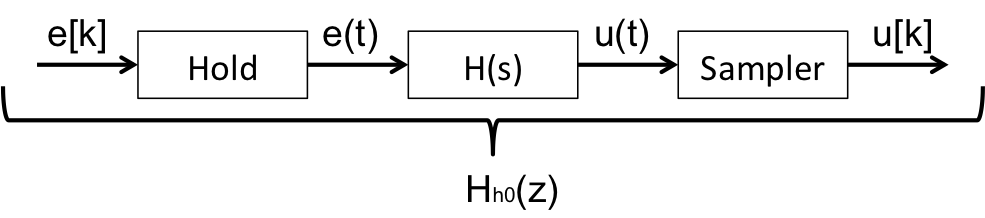
\includegraphics[width=0.8\linewidth]{hold_equivalent}
		\end{figure}
		\vspace{-1em}
		There are many techniques for holding a sequence of samples.
	\end{block}
\end{frame}

\begin{frame}
	\frametitle{Impuls-invariant method}
	\begin{block}{Practical rule}
		This method converts a continuous system into a discrete one by matching the impulse response using these transformations.
		\vspace{-1em}
		\begin{figure}
			\centering
			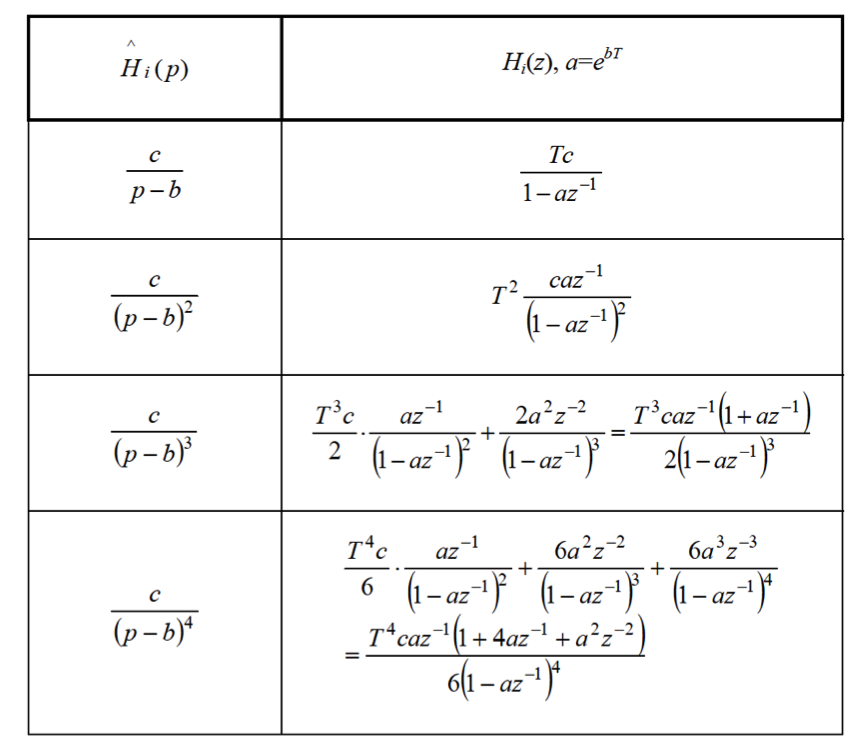
\includegraphics[width=0.5\linewidth]{impuls_inv}
		\end{figure}
	\end{block}
\end{frame}

\begin{frame}
	\frametitle{Zero-order hold equivalent (ZOH)}
\begin{columns}
	\begin{column}{0.5\textwidth}
	\begin{block}{Practical rule}
		The zero-order hold equivalent transfer function $H_{zoh}(z)$ can be found by computing the following:
		\begin{center}
			$H_{zoh}(z) = (1 - z^{-1}) \mathcal{Z}\{\frac{H(s)}{s}\}$
		\end{center}
		This rule is also called the Step-invariant method because it matches the step response of the continuous and the discrete system.
	\end{block}
	\end{column}
	
	\begin{column}{0.5\textwidth}
		\begin{figure}
			\centering
			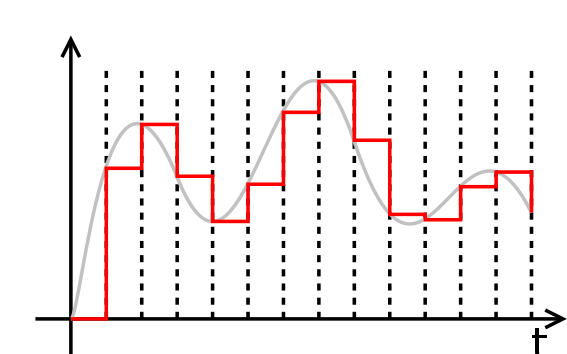
\includegraphics[width=1\linewidth]{zero-order}
		\end{figure}
	\end{column}
\end{columns}
\end{frame}

\begin{frame}
	\frametitle{Zero-order hold equivalent}
	\begin{example}
		\begin{center}
			$H(s) = \frac{0.1}{s + 0.1}$
		\end{center}
		Step 1: multiply by 1/s and perform partial fraction expansion
		\begin{center}
			$\frac{H(s)}{s} = \frac{0.1}{s * (s + 0.1)} = \frac{1}{s} - \frac{1}{s + 0.1}$
		\end{center}
		Step 2: perform z-transformation
		\begin{center}
			$\mathcal{Z} \{\frac{H(s)}{s}\} = \frac{1}{1 - z^{-1}} - \frac{1}{1 - e^{-0.1T} * z^{-1}}$
		\end{center}
		Step3: simplify and multiply by $(1-z^{1})$
		\begin{center}
			$H_{ho}(z) = \frac{1 - e^{-0.1T}}{z - e^{0.1T}}$
		\end{center}
	\end{example}
\end{frame}

\begin{frame}
	\frametitle{Zero-order hold equivalent}
	\begin{block}{Step Invariant Transformation}
		Zero-order hold equivalent of continuous systems with common transfer functions can easily be found by these transformations.
		\vspace{-1em}
		\begin{figure}
			\centering
			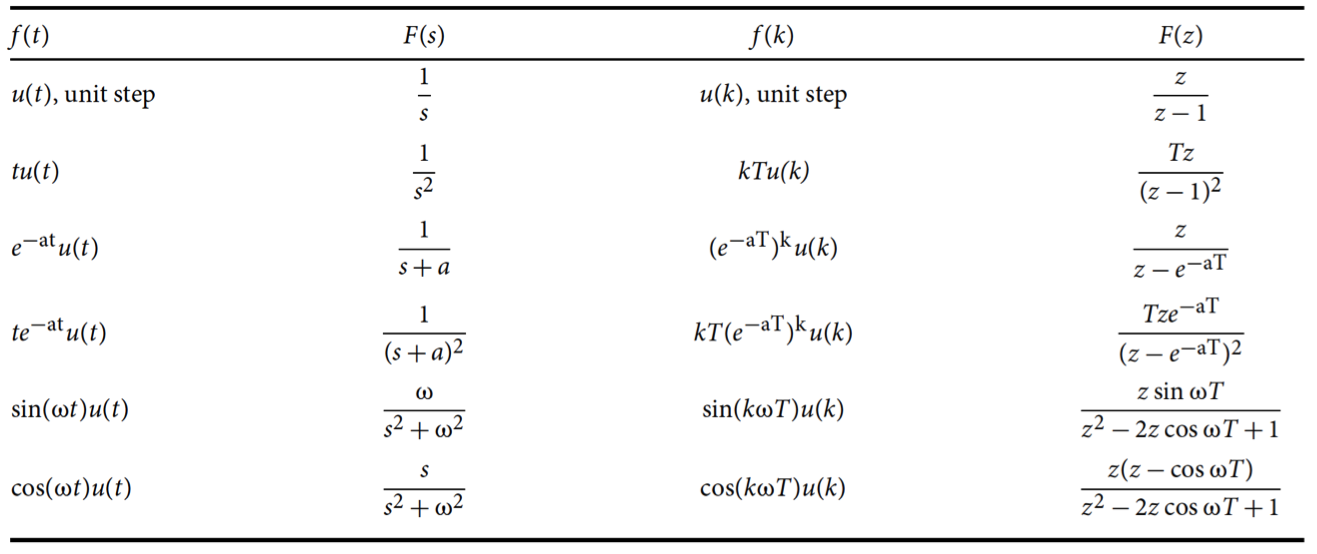
\includegraphics[width=1\linewidth]{step_inv}
		\end{figure}
	\end{block}
\end{frame}

\begin{frame}
	\frametitle{Non-causal first-order (= Triangle-hold equivalent (TRI))}
\begin{columns}
	\begin{column}{0.5\textwidth}
	\begin{block}{Practical rule}
		The non-causal first-order hold equivalent transfer function $H_{tri}(z)$ can be found by computing the following:
		\begin{center}
			$H_{tri}(z) = \frac{(z-1)^{2}}{Tz} \mathcal{Z}\{\frac{H(s)}{s^{2}}\}$
		\end{center}
	\end{block}
	
	\begin{alertblock}{Non-causal vs causal}
		A causal first-order hold equivalent introduces a time-delay resulting in a less accurate approximation.
	\end{alertblock}
	\end{column}
	
	\begin{column}{0.5\textwidth}
		\begin{figure}
			\centering
			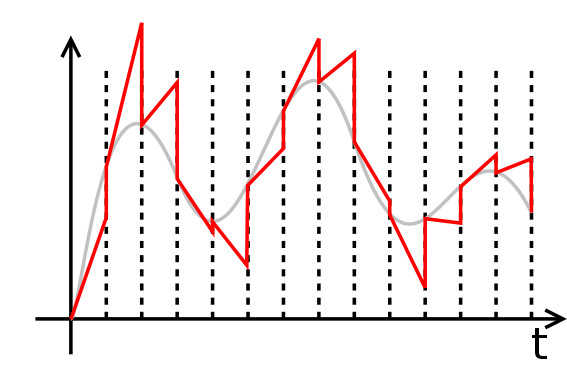
\includegraphics[width=1\linewidth]{first-order}
		\end{figure}
	\end{column}
\end{columns}
\end{frame}

\begin{frame}
	\frametitle{Triangle-hold equivalent}
	\begin{example}
		\begin{center}
			$H(s) = \frac{1}{s^{2}}$
		\end{center}
		Step 1: multiply by $1/s^{2}$ and perform partial fraction expansion
		\begin{center}
			$H(s) = \frac{1}{s^{4}}$
		\end{center}
		Step 2: perform z-transformation
		\begin{center}
			$\mathcal{Z}\{\frac{H(s)}{s^{2}}\} = \frac{T^{3}}{6} \frac{(z^{2} + 4z +1) z}{(z-1)^{4}}$
		\end{center}
		Step 3: simplify and multiply by $\frac{(z-1)^{2}}{T*z}$
		\begin{center}
			$H_{tri}(z) = \frac{T^{2}}{6} \frac{z^{2} + 4z + 1}{(z-1)^{2}}$
		\end{center}
	\end{example}
\end{frame}

\begin{frame}
	\frametitle{Effect of zero- and first-order hold equivalents}
	\begin{block}{Effects on the spectrum}
		Some information will be permanently lost.
		\vspace{-0.7em}
		\begin{figure}
			\centering
			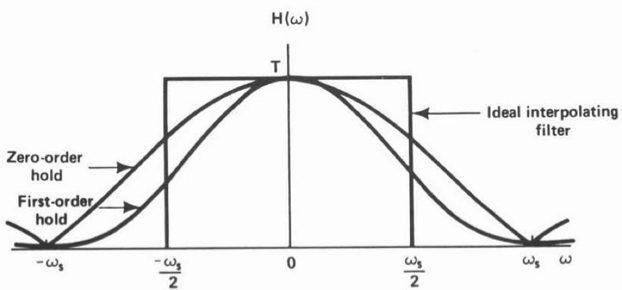
\includegraphics[width=1\linewidth]{effect_zoh_foh}
		\end{figure}
	\end{block}
\end{frame}

\section{Sampling Time}

\begin{frame}
	\frametitle{Sampling time $T_s$ based on the time response}
\begin{columns}
	\begin{column}{0.5\textwidth}
	\begin{block}{Rise time}
		Time needed to reach the steady state for the first time.
	\end{block}
	\begin{block}{Practical rule}
		A good rule of thumb is $T_s = T_{rising}/10$ seconds/sample.
	\end{block}
	\end{column}
	
	\begin{column}{0.5\textwidth}
		\begin{figure}
			\centering
			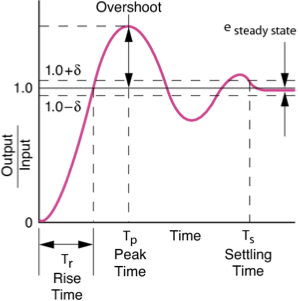
\includegraphics[width=1\linewidth]{rise_time}
		\end{figure}
	\end{column}
\end{columns}
\end{frame}

\begin{frame}
	\frametitle{Sampling time $T_s$ based on the frequency response}
	\begin{block}{Nyquist-Shannon sampling theorem}
		If a function $x(t)$ contains no frequencies higher than B hertz, it is completely determined by giving its ordinates at a series of points spaced $1/(2B)$ seconds apart. A sufficient sample-rate is therefore \textbf{2B samples/second}. This is called the \textbf{"Nyquist sampling rate"}. Equivalently, for a given sample rate $f_s$, perfect reconstruction is guaranteed possible for a bandlimit $B ≤ f_s/2$. A higher sampling rate creates a margin of error.
	\end{block}
	\begin{block}{Practical rule}
		A good rule of thumb is $T_s = 1/(2,2B)$ seconds/sample.
	\end{block}
\end{frame}

\section{Discretization and MATLAB}
\subsection{Calculation}
\begin{frame}
	\frametitle{MATLAB}
	\begin{block}{MATLAB Commands}
		MATLABs Control System Toolbox™ offers extensive support for discretization and resampling of linear systems:
	\begin{itemize}
		\item "c2d(system,sampling time,method)" used for discretization
		\item "d2c(system,sampling time,method)" used for reconstruction
		\item "d2d(system,sampling time,method)" used for resampling
	\end{itemize}
	\vspace{1em}
		These commands can also have extra options. It is necessary to specify the options in an additional command:
		"c2dOptions('OptionName',OptionValue)".
	\end{block}
\end{frame}

\begin{frame}
	\frametitle{MATLAB}
	\begin{block}{Available options}
		\begin{itemize}
			\item 'Method'
			\item 'PrewarpFrequency'
			\item 'FractDelayApproxOrder'
		\end{itemize}
	\end{block}
	
	\begin{block}{Available methods}
		\begin{itemize}
			\item zero-order hold equivalent: "zoh"
			\item first-order hold equivalent: "foh"
			\item impuls invariant rule: "impuls"
			\item zero-pole matching equivalent: "matched"
			\item bilinear: "tustin"
		\end{itemize}
	\end{block}
\end{frame}

\begin{frame}
	\frametitle{Exercise 1 with MATLAB}
	\begin{block}{Exercise 1}
		We will now discuss 4 methods applied on the same continuous system:
		$H(s) = \frac{s + 1}{s^{2} + s + 1}$\\
		\begin{itemize}
		\item The sampling time can be determined by the rule of thumb previously explained: $T_s$ = 2.2Bandwidth;
		\item MATLAB can calculate the bandwidth of a given continuous system, using the command: "bandwidth(system)".
		\end{itemize}
		This results in a sampling time of 0.25033 seconds for the given system
	\end{block}
\end{frame}

\begin{frame}
	\frametitle{Zero-order hold equivalent}
	\begin{example}
		Given:\\
		$H(s) = \frac{s + 1}{s^{2} + s + 1}$\\
		Sampling time = 0.25033sec\\
		\vspace{0.8em}
		MATLAB commands:
		
		H = tf([1 1],[1 1 1]) \\
		Hd = c2d(H,$0.25033$,'zoh')\\
		\vspace{0.8em}
		Result:
		$Hd_{zoh}(z) = \frac{0.2479z - 0.1927}{z^{2} -1.723z + 0.7785}$
	\end{example}
\end{frame}

\begin{frame}
	\frametitle{First-order hold equivalent}
	\begin{example}
		Given:\\
		$H(s) = \frac{s + 1}{s^{2} + s + 1}$\\
		Sampling time = 0.25033sec\\
		\vspace{1em}
		MATLAB commands:
	
		H = tf([1 1],[1 1 1]); \\
		Hd = c2d(H,$0.25033$,'foh')\\
		\vspace{1em}
		Result:
		$Hd_{foh}(z) = \frac{0.1245z^{2} + 0.02752z - 0.09691}{z^{2} - 1.723z + 0.7785}$
	\end{example}
\end{frame}

\begin{frame}
	\frametitle{Impuls invariant rule}
	\begin{example}
		Given:\\
		$H(s) = \frac{s + 1}{s^{2} + s + 1}$\\
		Sampling time = 0.25033sec\\
		\vspace{1em}
		MATLAB commands:
		
		H = tf([1 1],[1 1 1]); \\
		Hd = c2d(H,$0.25033$,'impuls')\\
		\vspace{1em}
		Result:
		$Hd_{impuls}(z) = \frac{0.2503z^{2} - 0.1883z}{z^{2} - 1.723z + 0.7785}$
	\end{example}
\end{frame}

\begin{frame}
	\frametitle{Zero-pole equivalent}
	\begin{example}
		Given:\\
		$H(s) = \frac{s + 1}{s^{2} + s + 1}$\\
		Sampling time = 0.25033sec\\
		\vspace{1em}
		MATLAB commands:
		
		H = tf([1 1],[1 1 1]); \\
		Hd = c2d(H,$0.25033$,'matched')\\
		\vspace{1em}
		Result: 
		$Hd_{matched}(z) = \frac{0.249z - 0.1939}{z^{2} - 1.723z + 0.7785}$
	\end{example}
\end{frame}

\begin{frame}
	\frametitle{Exercise 2 with MATLAB}
	\begin{block}{Exercise 2}
		We will now apply the bilinear rule with and without prewarping on the same continuous system: $H(s) = \frac{s^{2} + 0.5s + 9}{s^{2} + 5s + 1}$\\
		\vspace{0.5em}
		Criteria: 
		\begin{enumerate}
			\item The sampling time is chosen to be 0.5 seconds;\\
			\item The discrete system must have the same resonance frequency as the continuous one. MATLAB can calculate the resonance frequency: "damp(system)".
		\end{enumerate}
		\vspace{0.5em}
		The last criteria applies to this specific exercise. It is possible that the parity of the magnitude, of the discrete and the continuous system, at a different frequency (e.g. the peak frequency) is required.
	\end{block}	
\end{frame}
		
\begin{frame}
	\frametitle{Tusting rule}
	\begin{example}
		Given:\\
		$H(s) = \frac{s^{2} + 0.5s + 9}{s^{2} + 5s + 1}$\\
		Sampling time = 0.5sec\\
		\vspace{1em}
		MATLAB commands:
		
		H = tf([1,0.5,9],[1,5,9]) \\
		Hdt = c2d(H,0.5,'tustin')\\
		\vspace{1em}
		Result: 
		$Hd_{Tustin}(z) = \frac{0.6z^{2} - 0.3111z + 0.5111}{z^{2} -  0.3111z + 0.1111}$
	\end{example}
\end{frame}

\begin{frame}
	\frametitle{Tustin rule with prewarping}
	\begin{example}
		Given:\\
		$H(s) = \frac{s^{2} + 0.5s + 9}{s^{2} + 5s + 1}$\\
		Sampling time = 0.5sec\\
		\vspace{1em}
		MATLAB commands:\\
		H = tf([1,0.5,9],[1,5,9])\\
		damp(H) (results in 3.0Hz)\\
		discopts = c2dOptions('Method','tustin','PrewarpFrequency',3.0);\\
		Hdtp = c2d(H,0.5,discopts)\\
		\vspace{1em}
		Result:
		$Hd_{TustinPrewarp}(z) = \frac{0.5915z^{2} - 0.07726z + 0.5007}{z^{2} - 0.07726z + 0.09215}$
	\end{example}
\end{frame}

\subsection{Visualization}
\begin{frame}
	\frametitle{MATLAB}
	\begin{block}{MATLAB Commands for visualisation}
		\begin{itemize}
			\item MATLAB can draw the bode plots of the continuous system\\ 
			$\rightarrow$ command: "bode(system)"
			\item MATLAB can carry out a graphic showing the step response of the continuous system and the discretized system\\
			$\rightarrow$ command: "step(H,'b',Hd,'r')" in which 'b' and 'r' stand for blue and red. By using colors, the step responses of both systems can easily be distinguished
		\end{itemize}
		The following figures are a graphic representation of the exercises in MATLAB.
	\end{block}
\end{frame}

\begin{frame}
	\frametitle{Exercise 1: Zero-order hold equivalent}
	\vspace{-0.7em}
	\begin{figure}
		\centering
		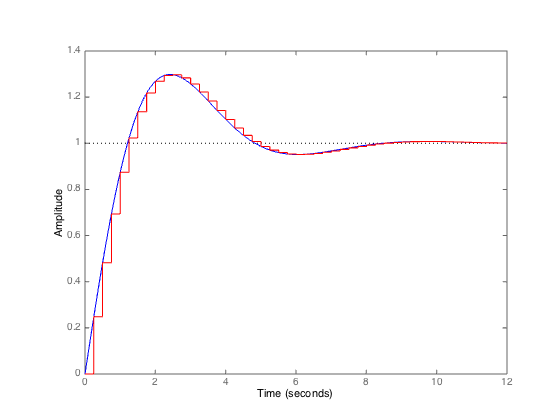
\includegraphics[width=0.8\linewidth]{vb1}
	\end{figure}
\end{frame}

\begin{frame}
	\frametitle{Exercise 1: First-order hold equivalent}
	\vspace{-0.7em}
	\begin{figure}
		\centering
		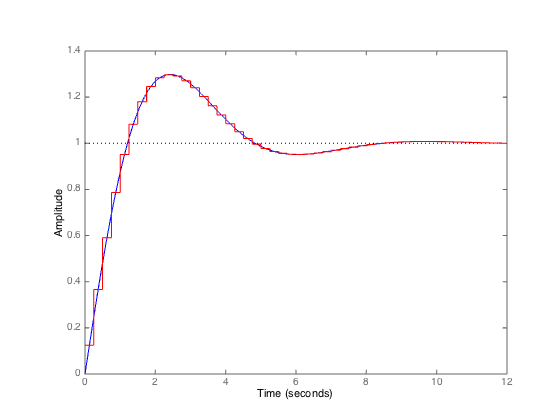
\includegraphics[width=0.8\linewidth]{vb2}
	\end{figure}
\end{frame}

\begin{frame}
	\frametitle{Exercise 1: Impuls invariant rule}
	\vspace{-0.7em}
	\begin{figure}
		\centering
		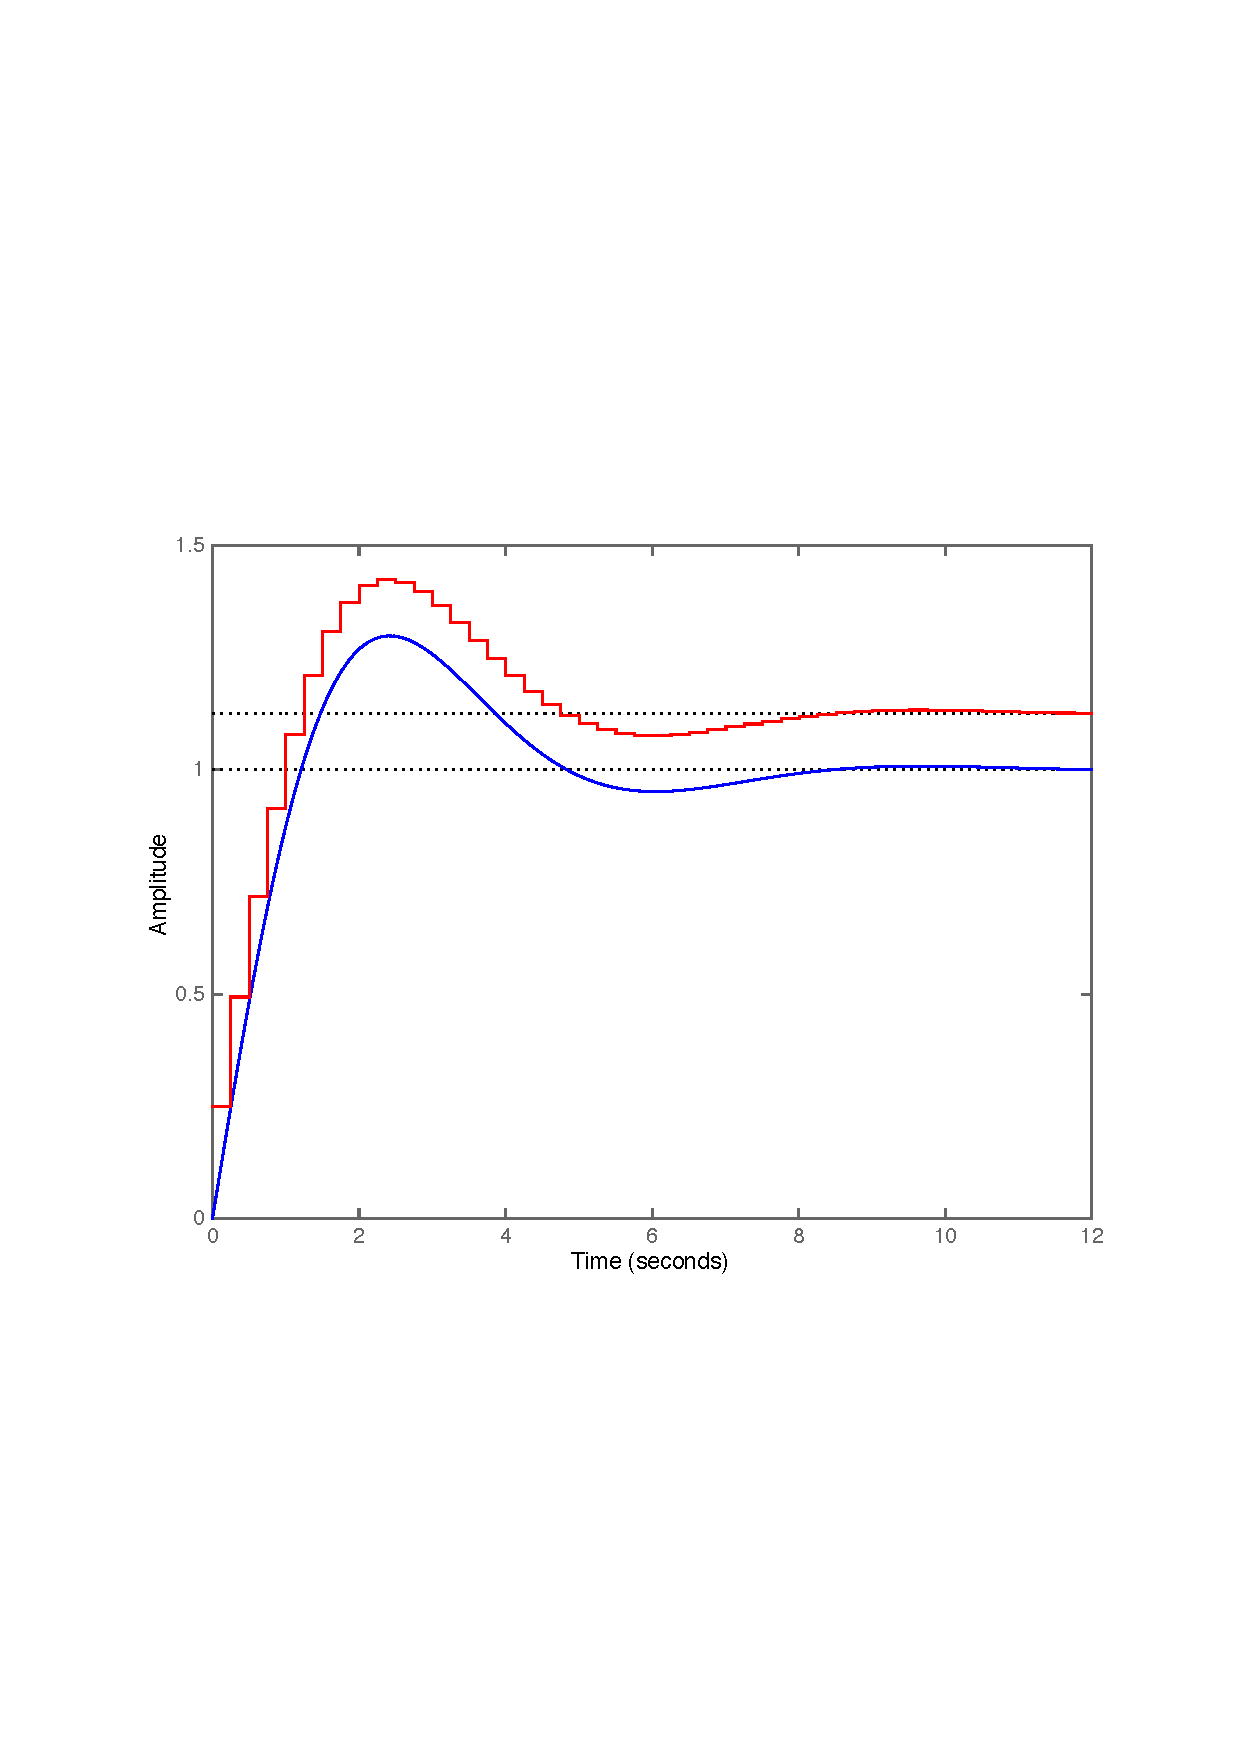
\includegraphics[width=0.8\linewidth]{vb3}
	\end{figure}
\end{frame}

\begin{frame}
	\frametitle{Exercise 1: Zero-pole equivalent}
	\vspace{-0.7em}
	\begin{figure}
		\centering
		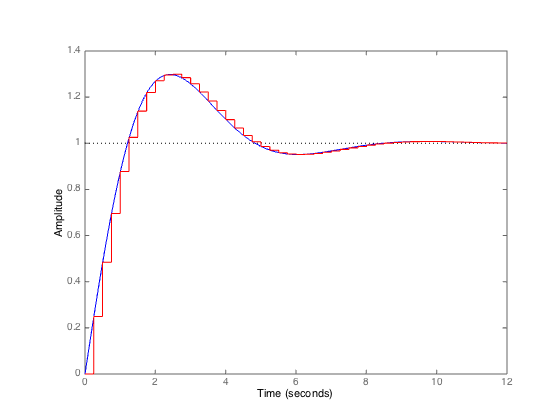
\includegraphics[width=0.8\linewidth]{vb4}
	\end{figure}
\end{frame}

\begin{frame}
	\frametitle{Exercise 2: Tustin rule}
	\vspace{-0.7em}
	\begin{figure}
		\centering
		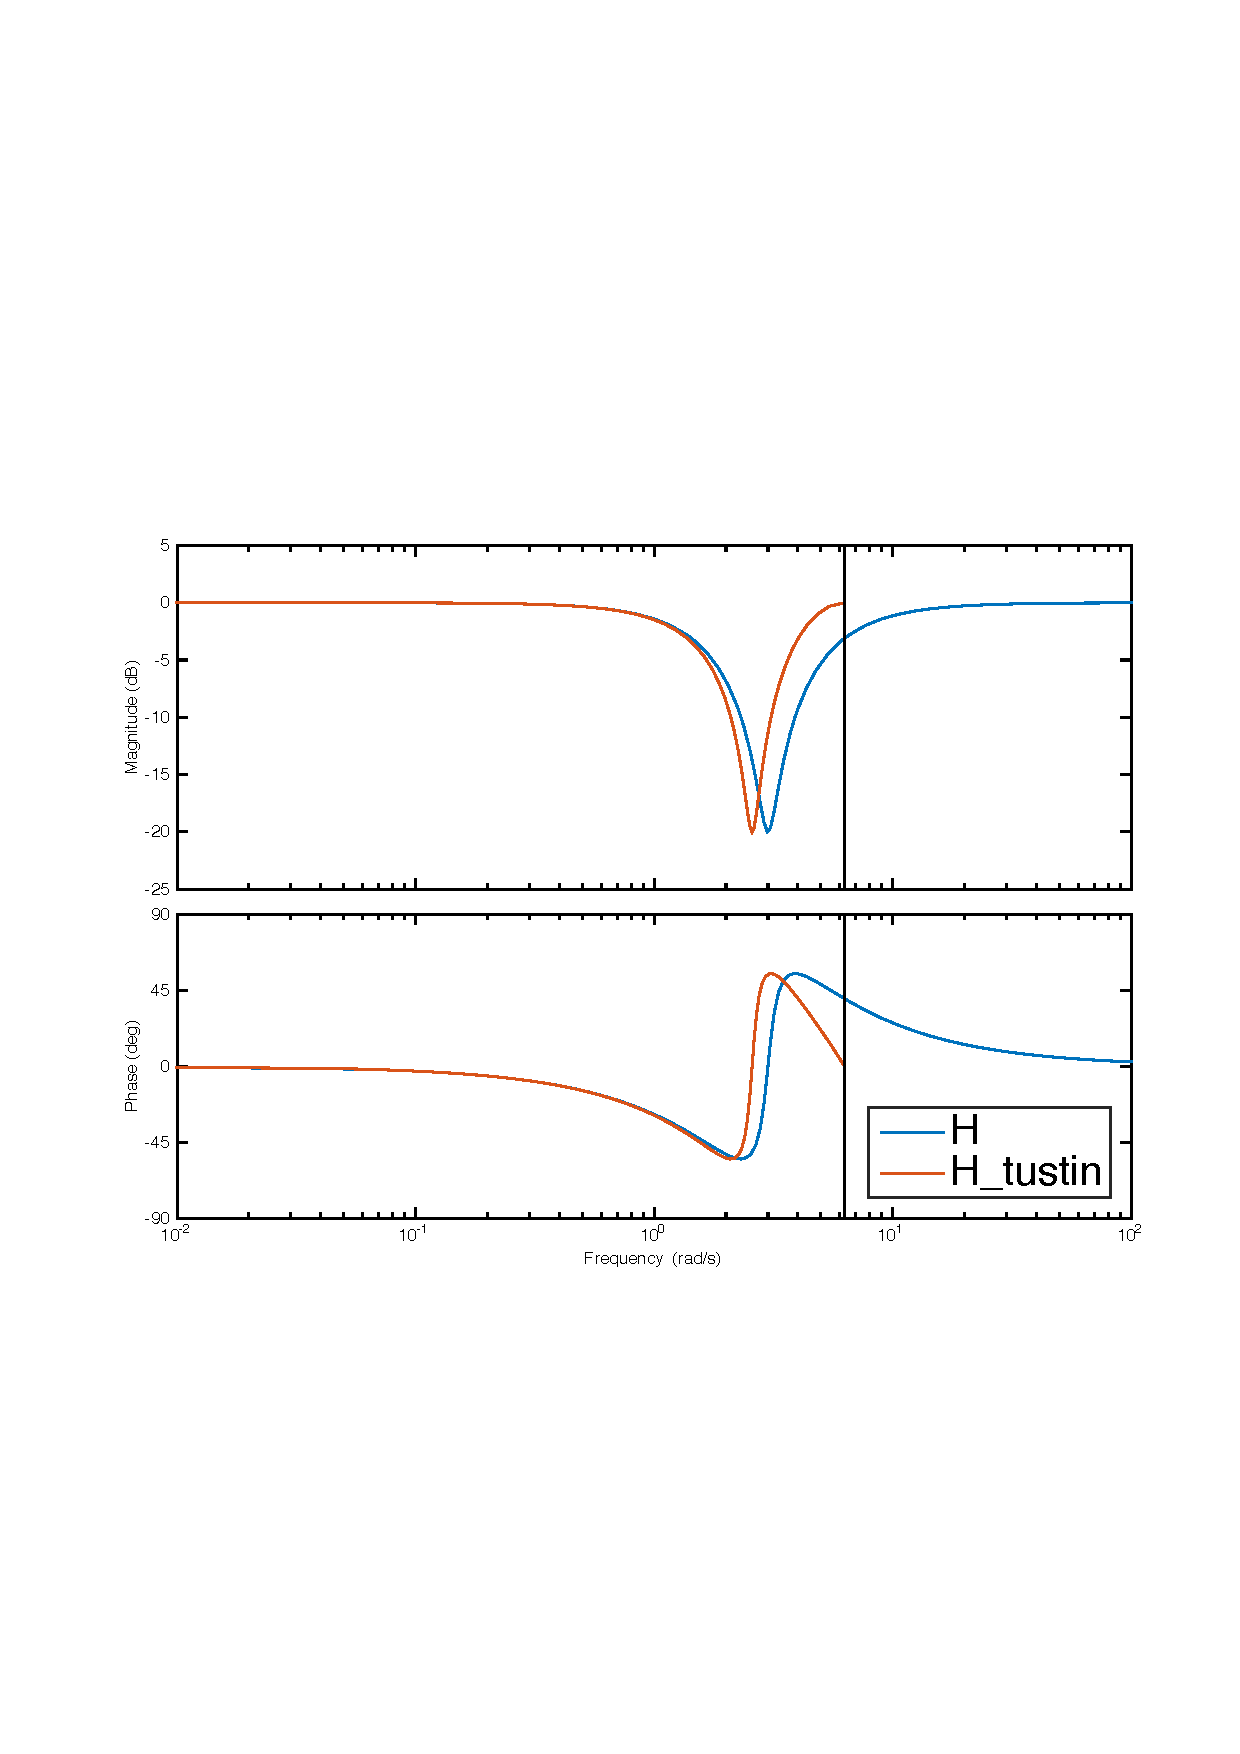
\includegraphics[width=0.9\linewidth]{distortion_bode2}
	\end{figure}
\end{frame}

\begin{frame}
	\frametitle{Exercise 2: Tustin rule with prewarping}
	\vspace{-0.7em}
	\begin{figure}
		\centering
		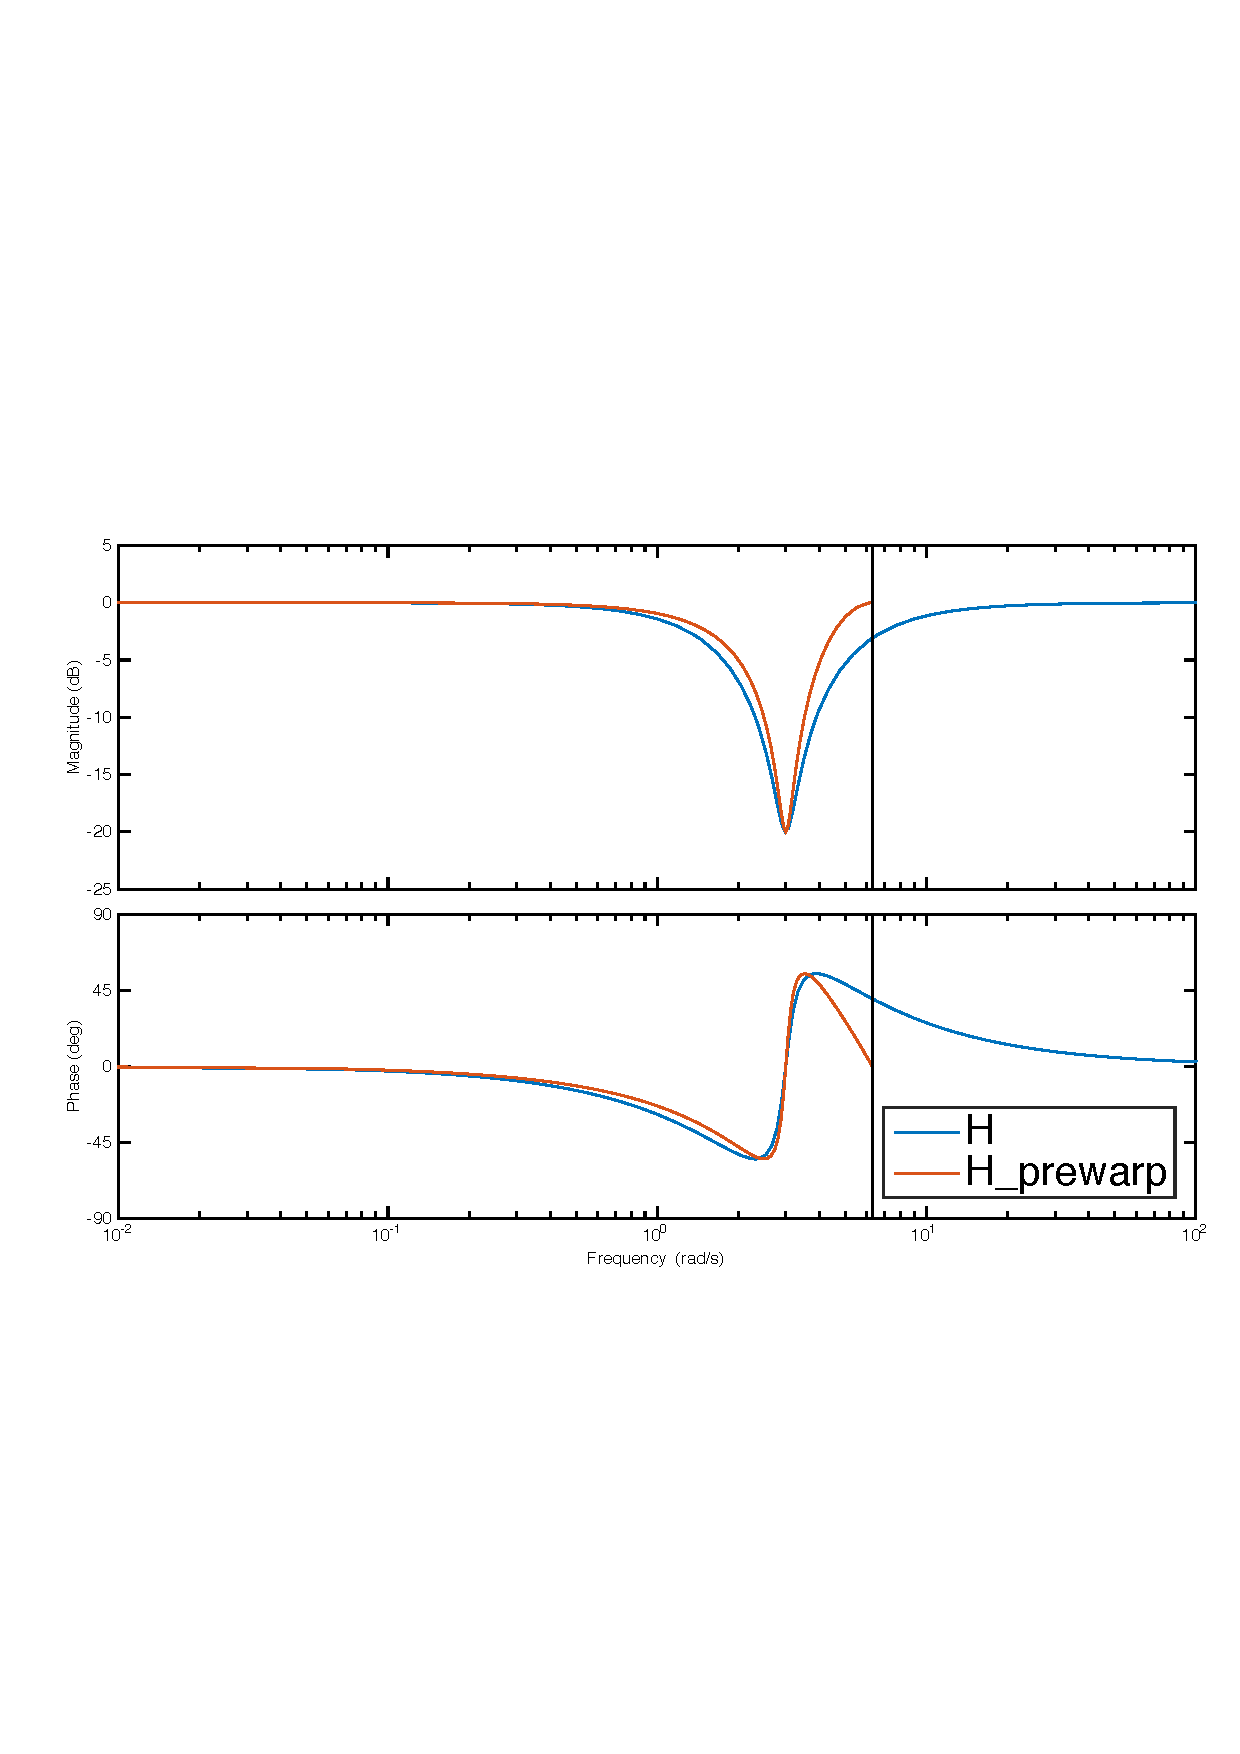
\includegraphics[width=1\linewidth]{distortion_bode3}
	\end{figure}
\end{frame}